\documentclass[a4paper]{scrreprt}

\usepackage{tikz}
\usetikzlibrary{positioning,calc}

\usepackage{lmodern}
\usepackage{microtype}
\usepackage[utf8]{inputenc}
\usepackage[T1]{fontenc}

\usepackage{amsmath}
\usepackage{amssymb}
\usepackage{amsfonts}
\usepackage[amsmath,amsthm,thref]{ntheorem}
\usepackage[retainorgcmds]{IEEEtrantools}

\usepackage{makeidx}
\usepackage{booktabs}
\usepackage{array}
\usepackage{float}
\usepackage{bbold}

\title{Galois Theory}
\author{Wenda Zhou}

\newcommand{\RR}{\mathbb{R}}
\newcommand{\EE}{\mathbb{E}}
\newcommand{\ZZ}{\mathbb{Z}}
\newcommand{\PP}{\mathbb{P}}

\newcommand{\mpunct}[1]{\, {#1}}

\newcommand{\Poisson}{\text{Poisson}}
\newcommand{\Normal}{\mathcal{N}}
\newcommand{\Bernouilli}{\text{Bernouilli}}
\newcommand{\Uniform}{\mathcal{U}}

\newcommand{\iid}{i.i.d. }
\newcommand{\pmf}{probability mass function }
\newcommand{\given}{\mid}

\newcommand{\indicator}[1]{\mathds{1}\left(#1\right)}

\newcommand{\curlyX}{\mathscr{X}}


%%% Local Variables: 
%%% mode: latex
%%% TeX-master: "statistics"
%%% End: 

\newtheorem{definition}{Definition}
\newtheorem{proposition}[definition]{Proposition}
\newtheorem{lemma}[definition]{Lemma}
\newtheorem{theorem}[definition]{Theorem}

%%% Local Variables: 
%%% mode: latex
%%% TeX-master: "Galois"
%%% End: 


\newcolumntype{V}{>{\centering\arraybackslash} m{0.4\linewidth}}

\makeindex

\begin{document}

\maketitle


\chapter{Estimation}

\section{Introduction}
\label{sec:1.1}

The course exposes some of the theory and methods of statistics \textemdash{} the science of making sense of data. Statistics can be directly applied to areas such as: market research, clinical trials, environment, finance, chemical experiments, government, sport etc.

In a typical problem of statistical inference, we have data which we regard as being generated from some unknown probability model. We aim to use the data to learn about the underlying model. Mathematically, let $X$ be a random variable taking values in a set $\curlyX$, and suppose that the distribution of $X$ belongs to a family of distributions indexed by a parameter $\theta$ taking values in a parameter space $\Theta \subseteq \RR^d$ (a parametric family).

\begin{example}
Consider the following parametric families and their parameter spaces.
\begin{itemize}
\item  $X \sim \Poisson (\mu)$, $\theta = \mu$, $\Theta = (0, \infty)$.
\item $X \sim \Normal(\mu, \sigma^2)$, $\theta = (\mu, \sigma^2)$, $\Theta = \RR \times (0, \infty)$.
\end{itemize}
\end{example}

Let $X1, \dotsc, X_n$  be independent identically distributed (i.i.d) random variables with the same distribution as $X$, so $\vec{X} = \left(X_1, \dotsc, X_n\right)$ is a simple random sample\index{random sample} (our data). We use the observed values $\vec{x}$ of $\vec{X}$ to make statistical inferences about $\theta$ such as:
\begin{enumerate}
\item giving an estimate $\hat{\theta} = \hat{\theta}(\vec{x})$ of the value of the true $\theta$ (point estimation).
\item giving an interval estimate $\left(\hat{\theta}_1(\vec(x)), \hat{\theta}_2(\vec(x))\right)$ for $\theta$.
\item testing a hypothesis such as $H: \theta \in \Theta_0$ where $\Theta_0 \subseteq \Theta$.
\end{enumerate}

\section{Probability review}
\label{sec:1.2}

\emph{See handout}

Note for calculation of $M_{Z_i^2}(t)$ in 6.d:
\begin{IEEEeqnarray*}{rCl}
M_{Z_i^2}(t) = \EE [e^{Z_i^2t}] &=& \int_0^\infty e^{z^2t}\frac{1}{\sqrt{2*\pi}}e^{-z^2/2} \d z \\
 &=& \int_{-\infty}^\infty \frac{1}{\sqrt{2\pi}} e^{-\frac{(1-2t)z^2}{2}} \d z \\
 &=& \sqrt{\frac{1}{1-2t}} \int_{-\infty}^\infty \frac{1}{\sqrt{2\pi\frac{1}{1-2t}}} e^{-\frac{1}{2\frac{1}{1-2t}}z^2} \d z
\end{IEEEeqnarray*}

\section{Estimation and bias}
\label{sec:1.3}

Suppose $X_1, \dotsc, X_n$ are i.i.d, each with probability density function (p.d.f.) or probability mass function (p.m.f.) $f(x ; \theta)$, where $\theta \in \Theta \subseteq \RR^d$ is unknown. We aim to estimate the value of $\theta$ by a (measurable) function $T(\dot)$ of the data. If $\vec{X}$ takes the value $\vec{x} = (x_1, \dotsc, x_n)$, then our estimate of $\theta$ is $\hat{\theta} = T(\vec{x})$. Note that $T$ does not involve $\theta$. $T(\vec{X})$ is our estimator\index{estimator} for $\theta$, and is a random quantity. The distribution of $T = T(\vec{X})$ is called its sampling distribution\index{sampling distribution}.

\begin{definition}
  An estimator $T(\vec{X})$ is unbiased\index{unbiased} for $\theta$ if $\forall \theta \in \Theta, \, \EE_\theta \left[T(\vec{X})\right] = \theta$. Otherwise, it is biased\index{biased}. Here $\EE_\theta$ is the expectation if $X_i$ has p.d.f/p.m.f $f(x ; \theta)$. The bias\index{bias} of $T(\vec{X})$ is $\EE_\theta\left[T(\vec{X})\right] - \theta$.
\end{definition}

%%% Local Variables:
%%% mode: latex
%%% TeX-master: "statistics"
%%% End:

\section{Conformal mappings}

\begin{definition}
  $f$ is conformal\index{conformal} at $w$ if $f$ is holomorphic at $w$ and $f'(w) \neq 0$.
\end{definition}

Note that if $f$ is conformal at $w$, then by the inverse function theorem, $f$ is locally bijective, and the local inverse function is conformal.

Two open sets $U$, $V$, related by a conformal bijection are said to be conformally equivalent\index{conformally equivalent}.

Viewing $f$ as a map $R^2 \rightarrow R^2$, then $f$ is locally invertible if $\det Df \neq 0$. Here, we have that $\det Df = u_xv_y - v_xu_y = u_x^2 + u_y^2$ (by the Cauchy-Riemann equations), hence we have that $f'(z) \neq 0$ implies that $\det Df > 0$. Note that this means that the map also preserves orientation.

Conformal maps preserve angles. Let $f$ be holomorphic on $U$. At $w \in U$, take two paths:
\[
g_i : [-1 ; 1] \rightarrow U, \gamma_i(0) = w, \gamma_i \text { differentiable (at 0). }
\]
Then we define the angle between $\gamma_1$ and $\gamma_2$ as:
\[
\text{angle}\left(\gamma_1, \gamma_2\right) = \arg \left(\gamma_1'(0)\right) - \arg \left(\gamma_2'(0)\right) \mpunct{.}
\]
Then, the paths are transformed under $f$ to $f \circ \gamma_i : [-1, 1] \rightarrow \CC$, and the angle becomes:
\[
\text{angle}\left(f \circ \gamma_1, f \circ \gamma_2\right) = \arg \left( (f \circ \gamma_1)'(0)\right) - \arg \left( (f \circ \gamma_2)'(0)\right) \mpunct{.}
\]
If $f$ is conformal at $w$, we have that:
\[
(f \circ \gamma_i)'(0) = f'\left(\gamma_i(0)\right)\gamma_i'(0) = f'(w)\gamma_i'(0)
\]
hence we can deduce that:
\[
\text{angle}\left(f \circ \gamma_1, f \circ \gamma_2\right) = \arg\left(\frac{\gamma_1'(0)}{\gamma_2'(0)}\right) = \text{angle}\left(\gamma_1, \gamma_2\right) \mpunct{.}
\]
Conformal maps preserve angles.

\paragraph{Example}

\begin{itemize}
\item Möbius maps $z \mapsto \frac{az+b}{cz+d}$, $ad - bc \neq 0$, from $\CC \cup \{ \infty \} \rightarrow \CC \cup \{ \infty \}$ are invertible, hence everywhere conformal.
\item The map $z \rightarrow z^n$ is everywhere homomorphic, and conformal except at $0$. This defines a conformal equivalence $\{ z \in \CC^* \mid 0 < \arg z < \pi/n \} \rightarrow \{ z \in \CC \mid Im z > 0 \}$.
\item The upper half plane is conformally equivalent to the open unit disk. Indeed, we have that $z \in H \Leftrightarrow \abs{z - i} < \abs{z + i} \Leftrightarrow \abs*{\frac{z-i}{z+i}} < 1$ (where $H$ denotes the upper half plane). So $z \rightarrow \frac{z-i}{z+i}$ takes $\{ \Im z > 0 \} \rightarrow \{ \abs{w} < 1 \}$. Note that since $f$ is the restriction of a Möbius map it is conformal.
\item The Jouhowski transformation\index{Jouhowski transformation}. Consider the map $z \mapsto w = \frac{1}{2}\left(z + \frac{1}{z}\right)$ (it can be proved that $\frac{w + 1}{w - 1} = \left(\frac{z + 1}{z - 1}\right)^2$). 
The map $f$ is holomorphic except at $0$, and the map is conformal (in $\CC^*$) except at $z = \pm 1$. 
In fact, we have that $f'(z) = 1 - \frac{z^2 + 1}{2z^2}$. If $z = re^{i\theta}$, and $w = u + iv$, $r, \theta, i, v \in \RR$, then we have:
\[
u = \frac{1}{2}\left(r + \frac{1}{r}\right)\cos \theta \text{ and } v = \frac{1}{2}\left(r + \frac{1}{r}\right)\sin \theta \mpunct{,}
\]
and hence a circle centered at the origin is mapped onto an ellipse:
\[
\{ \abs{z} = \rho \} \mapsto^f \left\{ \frac{u^2}{\frac{1}{4}\left(\rho + \frac{1}{\rho^2}\right)^2} + \frac{v^2}{\frac{1}{4}\left(\rho - \frac{1}{\rho}\right)^2} = 1 \right\} \mpunct{.}
\]
Now consider an off-centre circle through $-1$ and $-i$, then the image looks as follows [insert graph here], which is a crude approximation to an aerofoil. The Jouhowksi transformation can be used to transform fluid flow over a wing to understanding flow across a cylinder.
\end{itemize}

Observation: in building conformal equivalences by hand, it is often useful to describe a region bound by circular arcs as follows:
\[
\arg\left(\frac{z-\alpha}{z-\beta}\right) \in [\mu^+, \mu^-]
\]
\begin{figure}
  \centering
  \begin{tikzpicture}
    \tkzInit[xmin=-5,xmax=6]
    \tkzAxeX

    \tkzDefPoint(0,0){O}
    \tkzDefPoint(10,0){I}

    \tkzDefPoint(2, 2){C}
    \tkzDefShiftPoint[C](50:2){z}

    \tkzDefShiftPoint[C](10:2){alpha}
    \tkzDefShiftPoint[C](190:2){beta}

    \tkzDrawPoints(alpha,beta,z)


    \tkzDrawArc(C,alpha)(beta)
    \tkzDrawArc[style=dashed](C,beta)(alpha)

    \tkzInterLL(z,alpha)(O,I) \tkzGetPoint{iAlpha}
    \tkzInterLL(z,beta)(O,I) \tkzGetPoint{iBeta}

    \tkzDrawSegments(z,iAlpha z,iBeta)

    \tkzMarkAngle[fill=blue!25,mkpos=.2,size=0.5cm](I,iAlpha,alpha)
    \tkzMarkAngle[fill=green!25,mkpos=.2,size=0.5cm](O,iBeta,beta)
    \tkzMarkAngle[fill=red!25,mkpos=.2,size=0.5cm](beta,z,alpha)

    \tkzLabelPoint[above](z){$z$}
    \tkzLabelPoint[above right](alpha){$\alpha$}
    \tkzLabelPoint[left](beta){$\beta$}
    
    \tkzLabelAngle[pos=0.75](I,iAlpha,alpha){$\theta$}
    \tkzLabelAngle[pos=0.75](O,iBeta,beta){$\phi$}
    \tkzLabelAngle[pos=0.75](beta,z,alpha){$\mu$}
  \end{tikzpicture}
  \caption{Region bound by a circular arc}
  \label{fig:region_bound_by_circular_arc}
\end{figure}
As we can see in \cref{fig:region_bound_by_circular_arc}, as $z$ moves on the arc of circle, the angle $\mu$ is constant, and $\mu = \theta - \phi = \arg ( z - \alpha ) - \arg ( z - \beta )$.

\paragraph{Example}
The upper half of the open disk is conformally equivalent to the upper half plane $H$ and to the open unit disk. 
Consider the region $\{ z \mid \Im z > 0, \abs{z} < 1 \} = \{ z = \mid \pi/2 < \arg \left(\frac{z-1}{z+1}\right) < \pi\}$. Then the map $z \mapsto \frac{z-i}{z+1} = w$ takes $R$ to the upper left quadrant after which the map $w \mapsto -w^2$ maps the upper left quadrant to the upper half plane.

\paragraph{Riemann mapping theorem}
Let $D \subseteq \CC$ be any domain (open set) bound by a simple closed curve. Then there exisits a conformal bijection $\phi : D \rightarrow \{ \abs{z} < 1 \}$. In particular, the interior of the Koch snowflake is conformally equivalent to the unit disk.



%%% Local Variables: 
%%% mode: latex
%%% TeX-master: "complex_analysis"
%%% End: 

\begin{definition} \label{def:5}
  Let $L/K$ be an extension, and $\alpha \in L$ be algebraic over $K$. As $K[X]$ is a principal ideal domain, we have that:
  \begin{equation*}
    I_\alpha = (P_\alpha) = \{ \text{multiples of } \alpha \}
  \end{equation*}
  for a unique monic $P_\alpha \in K[X]$. This $P_\alpha$ is called the minimal polynomial\index{minimal polynomial} of $\alpha$ over K. 
\end{definition}
Note: $\text{deg} P_\alpha$ is minimal amongst $\text{deg} P$ for $P \neq 0, P \in I_\alpha$.

\subparagraph{Example}
\begin{itemize}
\item The minimal polynomial of $\alpha = \sqrt{2}$ over $\mathbb{Q}$
  \begin{equation*}
    P_\alpha = X^2 -2 \in \mathbb{Q}[X]
  \end{equation*}
\item The minimal polynomia of $\alpha = \sqrt{2}$ over $\mathbb{R}$ is 
  \begin{equation*}
    P_\alpha = X-\sqrt{2} \in \mathbb{R}[X]
  \end{equation*}
\item The minimal polynomial of $\alpha = \sqrt[3]{2}$ over $\mathbb{Q}$ is
  \begin{equation*}
    P_\alpha = X^3 - 2 \in \mathbb{Q}[X]
  \end{equation*}
\end{itemize}

Consider $f_\alpha : \mathbb{Q} \rightarrow \mathbb{C}$, and let $\mathbb{Q}(\alpha) = \text{Im} f_\alpha = \{ a + b\alpha + c\alpha^2 / a, b, c \in \mathbb{Q}\} \subseteq \mathbb{C}$. This is a field , as it is a ring and every non zero element is invertible. 

e.g. find the inverse of $(1+\alpha)$, use:
\begin{equation*}
  (1+\alpha)(1-\alpha+\alpha^2) = 1+\alpha^3 = 3
\end{equation*}
hence we have that
\begin{equation*}
  (1+\alpha)^{-1} = \frac{1}{3}(1-\alpha+\alpha^2)
\end{equation*}

\section{Simple extensions}
Note: the intersection of subfields is a subfield. However, the union of subfields are not subfields in general.

\begin{definition} \label{def:6}
  Let $L/K$ be an extension and $\alpha \in L$. We denote by $K(\alpha)$ the intersection of all subfields of L, containing K and $\alpha$, i.e. the minimal such subfield. Then $K(\alpha)/K$ is called the extension generated\index{generated (extension} by $\alpha$. We say that $L/K$ is simple if it is generated by some $\alpha \in L$.
\end{definition}

\begin{proposition} \label{prop:7}
  Let $L/K$ be an extension and $\alpha \in L$. Then, we have that:
  \begin{enumerate}
  \item Its minimal polynomial is $P_\alpha$ over K is irreducible over $K[X]$.
  \item $\text{Im} f_\alpha = K(\alpha)$ and $[K(\alpha) : K] = \deg P_\alpha$. In particular, $K(\alpha)/K$ is finite.
  \end{enumerate}
\end{proposition}

\begin{proof} 
  \begin{enumerate}
  \item If $P_\alpha(X) = P(X)Q(X)$, then we have: $P(\alpha)Q(\alpha) = P_\alpha(\alpha) = 0$, hence $P(\alpha) = 0$ or $Q(\alpha) = 0$. Say $P(\alpha) = 0$, then $P \in I_\alpha$, i.e. $P_\alpha \mid P$, hence $Q$ is a unit $K[X]$.

  \item $\text{Im} f_\alpha$ is a subfield of $L$ 

It is certainly a ring as the image of a ring homomorphism. Every $x \in \text{Im}$ is of the form $P(\alpha)$ for some $P \in K[X]$. If $x \neq 0$, then we have that $P \not\in I_\alpha$, i.e. $P$ is not divisible by $P_\alpha$. Hence, $\exists Q \in K[X], with PQ \equiv 1 \mod{P_\alpha}$, therefore $P(\alpha)^{-1} = Q(\alpha) \in \text{Im} f_\alpha$.

  \item $\text{Im} f_\alpha = K(\alpha)$

As $\text{Im} f_\alpha$ is a subfiel of $L$ containing $K$ and $\alpha$, and every such field must contain $\text{Im} f_\alpha$. We have $\text{Im} f_\alpha = K(\alpha)$.

  \item If $\deg P_\alpha = n$, then $\{1, \alpha, \alpha^2, \ldots, \alpha^{n-1}\}$ gives a basis of $K(\alpha)$ as a vector space over K.

For every $x = P(\alpha) \in \text{Im} f_\alpha$, there exits $Q, E \in K[X]$ with $P = P_\alpha\cdot{}Q + R$ and $\deg R < n$ hence $x = P(\alpha) = R(\alpha)$ is a K-linear combination of $\{1, \alpha, \alpha^2, \ldots, \alpha^{n-1}\}$. If $R(\alpha) = 0$, with $\deg R < n$, then $P_\alpha \mid R$ by definition of the minimal polynomial, hence $R = 0$.
  \end{enumerate}
\end{proof}

\subparagraph{Remarks}
\begin{enumerate}
\item Different elements can generate the same field, i.e. we can have $K(\alpha) = K(\alpha')$ with $\alpha \neq \alpha'$, e.g.
  \begin{equation*}
    \mathbb{Q}(1+\sqrt{2}) = \mathbb{Q}(\sqrt{2})
  \end{equation*}

\item By \ref{prop:4} and \ref{prop:7} for an extension $L/K$ and $\alpha \in L$, then we have:
  \begin{equation*}
    \alpha \text{algebraic over K} \Leftrightarrow K(\alpha)/K \quad \text{is finite} 
  \end{equation*}

\item If $K \subseteq L \subseteq F$ and $\alpha \in F$, then $K[X] \subseteq L[X]$ implies:
  \begin{enumerate}
  \item if $\alpha$ algebraic over K, then $\alpha$ algebraic over L. Note that the converse holds when $L/K$ is finite.
  \item its minimal polynomial $Q_\alpha$ over L divides its minimal polynomial $P_\alpha$ over K.
  \end{enumerate} 

\item Related question:

We have that $\sqrt{2}$, $sqrt[3]{2}$ algebraic over $\mathbb{Q}$, does this imply $\sqrt{2} + \sqrt[3]{2}$ alebraic over $\mathbb{Q}$? Answer is yes, finding appropriate polynommail is left as an exercise for the reader.
\end{enumerate}

\section{Finite extensions}
\subparagraph{Note} if $[L : K] = 1$, then $L = K$ (as we have a 1-dimensional K-vector space).

\begin{proposition}[Tower Law]\label{prop:8}
  Let $K \subseteq L \subseteq F$, then if $L/K$, $F/L$ are finite extensions then so is $F/K$, and we have
  \begin{equation*}
    [F : K] = [F:L][L:K]
  \end{equation*}
\end{proposition}

\begin{proof}
  Let $\{a_1, \ldots, a_n \} \subseteq L$ be a basis of $L/K$ (i.e a basos of L as a vector space over K).
Let $\{ b_1, \ldots, b_m \}$ be a basis of $F/L$. Then every $x \in F$ is written as:
\begin{equation*}
  x = x_1b_1 + \ldots + x_mb_m
\end{equation*}
with $x_j \in L$ for $1 \leq j \leq m$, and each $x_j \in L$ is written as:
\begin{equation*}
  x_j = x_{1j}a_1 + \ldots + x_{nj}a_n
\end{equation*}
with $x_{ij} \in K$ for each $1 \leq i \leq n$, $1 \leq j \leq m$. Hence, we have that:
\begin{equation*}
  x = \sum_j\left(\sum_ix_{ij}a_i\right)b_j = \sum_{i, j}x_{ij}a_ib_j
\end{equation*}
If $x = \sum_{i, j}x_{ij}a_ib_j = 0$, then $\sum_j x_{ij}a_i = 0$ for all $j$ by the L-linear independence of $b_j$, therefore $x_{ij} = 0$ by K-linear independence of the $a_i$.

Thus, we have that the following is a basis of $F/K$:
\begin{equation*}
  \{ a_ib_j \mid 1 \leq i \leq n, 1 \leq j \leq m \}
\end{equation*}
\end{proof}






%%% Local Variables: 
%%% mode: latex
%%% TeX-master: "Galois"
%%% End: 

\begin{proof}
  By applying the chain rule to $e^{\log z} = z$, we find that $\frac{d}{dz}\log z = \frac{1}{z}$.

  We can check hat the given power series has radius of convergence $1$. We have that:
\[
\frac{d}{dz} \log (1+z) = \frac{1}{1+z}\mpunct{,}
\]
but we also have that:
\[
\frac{d}{dz}\left(\sum_{n\geq 1} (-1)^{n-1}\frac{z^n}{n}\right) = \frac{1}{1+z} \mpunct{.}
\]
Now evaluate at $0$ to check the expressions agree.
\end{proof}

\paragraph{Heuristic remark}

Instead of slitting the plane, one could view $\log$ as a multi-valued function $z \mapsto \{ \ln \abs{z} + i\theta \mid \theta \text{ is any value of } \arg z\}$. 
A point $p \in \CC$ such that the multi-valued function $f$ has no continuous single-value branch in any neighbourhood $B_\epsilon(p) \setminus \{p\}$ is called a branch point\index{branch point} of $f$.
For example, $0$ is a branch point of $\log$. We can set $z^\alpha = e^{\alpha\log z}$ and hence define for example $\sqrt{z}$ either as a function on a slit plane, or as a multi-valued function with branch point at $0$.
To resolve the problem of branch points, it is possible to say that $\log$, $z^{1/2}$ are well-defined on certain Riemann surfaces (spaces mapping to $\CC^*$).

\section{Contour integrals}
Let $f : [a, b] \rightarrow \CC$. We say $f$ is (Riemann) integrable\index{integrable} if $\Re f$ and $\Im f$ are integrable. We define
\[
\int_a^b f(t)dt = \int_a^b\Re f (t) dt + i\int_a^b \Im f(t) dt \mpunct{.}
\]

\begin{proposition}
\[
\abs*{\int_a^b f(t) dt} \leq (b-a)\sup_t\abs*{f(t)} \mpunct{,}
\]
with equality if and only if $f$ is constant.
\end{proposition}

\begin{proof}
  let $\theta = \arg \int_a^b f(t) dt$, and let $M = \sup\abs{f(t)}$. We have that:
\begin{IEEEeqnarray*}{rCl}
\abs*{\int_a^b f(t)} &=& \int_a^b e^{-i\theta}f(t) dt \\
&=& \int_a^b \Re (e^{-i\theta} f(t)) dt \quad \text{ as we know that the previous line is real} \\
&\leq& \int_a^b \abs{f(t)} dt \\
&\leq& (b-a)M \mpunct{.} 
\end{IEEEeqnarray*}
We have equality if and only if $\abs{f(t)} = M$ and $\arg f(t) = \theta$, i.e. $f$ is constant.
\end{proof}

\begin{definition}
  A path\index{path} is a $C^1$-smooth (or just smooth) map $\phi : [a, b] \rightarrow \CC$. A path is said to be simple\index{simple (path)} if there are no self-intersections except (possibly) at the end points, i.e.
\[
\phi(t_1) = \phi(t_2) \Rightarrow \{t_1, t_2\} = \{a, b\} \text{ or } t_1 = t_2 \mpunct{.}
\]
A simple closed path is called a contour\index{contour}.
\end{definition}

If $\gamma : [a, b] \rightarrow \CC$ is $C^1$-smooth, we let:
\[
\text{length}(\gamma) = \int_a^b \abs*{\gamma'(t)} dt\mpunct{.}
\]

\begin{definition}
  Given $\gamma : [a, b] \rightarrow U \subseteq \CC$  path, and $f : U \rightarrow \CC$ continuous, we define:
\[
\int_\gamma f(z) dz = \int_a^b f\left(\gamma(t)\right)\gamma'(t) dt
\]
\end{definition}

\paragraph{Easy properties}

\begin{enumerate}
\item Integrating along some fixed path $\gamma$ is linear in the function $f$.
\item If $-\gamma$ denotes the path $\gamma$ traversed in the opposite direction, then:
\[
\int_{-\gamma} f(z)dz = -\int_\gamma f(z) dz \mpunct{.}
\]

\item The integral along $\gamma$ is independent of the parametrisation of the path. 
Indeed, let $\phi : [a', b'] \rightarrow [a, b]$ be $C^1$ with $\phi(a') = a$ and $\phi(b') = b$. 
Then if $\delta = \gamma \circ \phi$, we claim:
\[
\int_\delta f(z) dz = \int_\gamma f(z) dz \mpunct{.}
\]
We have the following:
\[
  \int_{a'}^{b'} f(\gamma(\phi(t)))\gamma'(\phi(t))\phi'(t) dt = \int_a^b f(\gamma(u))\gamma'(u) du
\]
where we have set $u = \phi(t)$.
\end{enumerate}

\paragraph{Remark}

If $\gamma$ is only piecewise $C^1$ smooth, we define:
\[
\int_\gamma f(z)dz = \sum_i \int_{\gamma_i} f(z)dz 
\]
where $\gamma = \gamma_1 * \gamma_2 * \dotsb * \gamma_r$ is a concatenation of smooth $\gamma_i$. 
Integration is additive in the sense that, if $a < \tilde{a} < b$, then we have:
\[
\int_\gamma f(z)dz = \int_{\gamma\rvert_{[a, \tilde{a}]}} f(z)dz + \int_{\gamma\rvert_{[\tilde{a}, b]}} f(z) dz \mpunct{.}
\]

\paragraph{Example}

Let $f(z) = z^n$ defined on $U = \CC^*$, and let $\gamma : [0, 2\pi] \rightarrow U$ such that $\gamma(\theta) = e^{i\theta}$. Then, we have that:
\[
\int_\gamma f(z) dz = \begin{cases}2\pi{}i & \text{if } n = -1 \mpunct{,} \\0 & \text{otherwise.}\end{cases}
\]

\begin{proof}
  We have the following:
\[
\int_\gamma f(z)dz = \int_0^{2\pi}e^{in\theta}ie^{in\theta}d\theta = i\int_0^{2\pi} e^{i(n+1)\theta}d\theta \mpunct{.}
\]
Hence, if $n = -1$, we get $2\pi{}i$. If $n \neq -1$, we have that $\left[\frac{e^{i(n+1)\theta}}{n+1}\right]_0^{2\pi} = 0$.
\end{proof}

\paragraph{Example}
\begin{figure}
  \centering
   \begin{tikzpicture}[scale=0.75]
    \tkzInit[xmin=-5,xmax=5,ymin=-1,ymax=5]

    \tkzDefPoint(0,0){O}
    \tkzDefPoint(-4,0){A}
    \tkzDefPoint(4,0){B}

    \tkzDefPoint(-5,0){xmin}
    \tkzDefPoint(5,0){xmax}

    \tkzDefPoint(0,5){ymax}
    \tkzDefPoint(0,-1){ymin}

    \tkzDrawSegment(xmin,xmax)
    \tkzDrawSegment(ymin,ymax)

    \tkzDrawArc[color=blue](O,B)(A)
    \tkzDrawSegment[color=blue](B,A)

    \tkzLabelPoint[below](A){$-R$}
    \tkzLabelPoint[below](B){$R$}

  \end{tikzpicture}

  \caption{half-circle of radius $R$}
  \label{fig:4.1}
\end{figure}

Let $\gamma$ be as in the figure\ref{fig:4.1}, and $f(z) = z^2$. We write $\gamma = \gamma_1 * \gamma_2$, with $\gamma_1 : [-R, R] \rightarrow \CC$ such that $\gamma_1(t) = t$ and with $\gamma_2 : [0, 1] \rightarrow \CC$ such that $\gamma_2(t) = Re^{i\pi{}t}$.
Then we have the following:
\begin{IEEEeqnarray*}{rCl}
\int_\gamma f(z) dz &=& \int_{-R}^R t^2dt + \int_0^1 R^2e^{2\pi i t} i \pi R e^{i \pi t} dt \\
&=& \frac{2R^3}{3} + R^3 i \pi \int_0^1 e^{3\pi i t} dt \\
&=& \frac{2R^3}{3} - \frac{2R^3}{3} \\
&=& 0 \mpunct{.}
\end{IEEEeqnarray*}

\begin{proposition}
  For a path $\gamma : [a, b] \rightarrow U$ and $f : U \rightarrow \CC$ continuous, we have that:
\[
\abs*{\int_\gamma f(z) dz} \leq \text{length}(\gamma) \sup_\gamma \abs*{f(z)} \mpunct{.}
\]
\end{proposition}

\begin{proposition}
  Let $f : U \rightarrow \CC$ be continuous, and suppose that there exists $F : U \rightarrow \CC$ such that $F'(z) = f(z)$ for all $z \in U$. Then if $\gamma : [a, b] \rightarrow U$, we have that:
\[
\int_\gamma f(z) dz = F(\gamma(b)) - F(\gamma(a)) \mpunct{.}
\]
\end{proposition}

\begin{proof}
  We have that:
\[
\int_\gamma f(z) dz = \int_a^b f(\gamma(t))\gamma'(t) dt = \int_a^b(F \circ \gamma)'(t) dt \mpunct{.}
\]
\end{proof}

$F$ is called an antiderivative\index{antiderivative} of $f$ on $U$.

%%% Local Variables: 
%%% mode: latex
%%% TeX-master: "complex_analysis"
%%% End: 

\section{Cauchy's theorem}
By the Fundamental Theorem of Calculus, we know that if $f(z)$ has an antiderivative, then $\int_\gamma f(z) dz = 0$ for any $\gamma : [a, b] \rightarrow U$ closed (i.e. $\gamma(a) = \gamma(b)$.

\paragraph{Example}

Recall the example of $z^n$ integrated along $t \mapsto e^{it} \subseteq \CC^*$. If $n \neq -1$, we have that:
\[
f(z) = \frac{d}{dz}\left(\frac{z^{n+1}}{n+1}\right) = z^n \Rightarrow \int_\gamma z^n dz = 0 \mpunct{.}
\]
On the other hand, if $n = -1$, then we ave $f(z) = \frac{d}{dz}(\log z)$ on a slit plane. Such a slit plane does not contain $\gamma$. Indeed, we have that $\int_\gamma \frac{1}{z} dz \neq 0$.

\begin{proposition}
  If $f : U \rightarrow \CC$ is continuous, $U \subseteq \CC$ open and path connected, and if:
\[
\int_\gamma f(z) dz = 0 
\]
for any closed path $\gamma : [a, b] \rightarrow U$, then there exists an antiderivative $F$, holomorphic on $U$, with $F'(z) = f(z)$.
\end{proposition}

\begin{proof}
  Pick $a_0 \in U$. For each $w \in U$, pick a path$\gamma_w : [0, 1] \rightarrow U$ such that $\gamma_w(0) =  a_0$ and $\gamma_w(1) = w$. Now define $F$ as:
\[
F(w) = \int_{\gamma_w} f(z) dz \mpunct{.}
\]
Observe that the hypothesis $\int_\gamma f(z) dz = 0$ for closed paths $\gamma$ shows that the value of $F(w)$ does not depend on the choice of the path $\gamma_w$.

Now, let us prove that $F$ is holomorphic, with $F' = f$. Since $U$ is open, we have that for all $w \in U$, $\exists r > 0, B_w(r) \subseteq U$. Consider some point $w + h \in B_w(r)$, and let $\delta_h$ be the radial path from $w$ to $w+h$ inside the ball. If $\gamma = \gamma_w * \delta_h * (-\gamma_{w+h})$, then $\gamma$ is closed and $\int_\gamma f(z) dz = 0$. So we have the following:
\begin{IEEEeqnarray*}{rCl}
F(w+h) &=& \int_{\gamma_w * \delta_h} f(z) dz \\
&=& F(w) + \int_{\delta_h} f(z) dz \\
&=& F(w) + hF(w) + \int_{\delta_h} \left(f(z) - f(w)\right) dz \mpunct{.}
\end{IEEEeqnarray*}
Hence, we deduce that:
\begin{IEEEeqnarray*}{rCl}
  \abs*{\frac{F(w+h) - F(w)}{h} - f(w)} &=& \abs*{\frac{1}{h} \int_{\delta_h} \left(f(z) - f(w)\right) dz} \\
&\leq& \left(\frac{1}{\abs{h}} \text{length}(\delta_h)\right) \sup_{z \in \delta_h} \abs*{f(z) - f(w)} \mpunct{.}
\end{IEEEeqnarray*}
Now, the right-hand side tends to $0$ as $h$ tends to $0$ by continuity of $f$.
\end{proof}

Remark, suppose $U$ is not just path-connected, but convex, or star-shaped about $a_0$ (i.e. the radial path from $a_0$ to any point in $U$ is in $U$). 
Then, we could have taken $\gamma_w$ to be the straight line segment from $a_0$ to $w$ for every $w$. 
The previous proof only used that $\int_{\partial T} f(z) dz = 0$ where $T \subseteq U$ is a triangle, i.e. a contour made of three straight lines.

\begin{theorem}%[Cauchy's theorem for triangles]
  Let $U \subseteq \CC$ be an open path-connected set. Let $T \subseteq U$ be a triangle. If $f : U \rightarrow \CC$ is holomorphic, then we have:
\[
\int_{\partial T} f(z) dz = 0 \mpunct{.}
\]
\end{theorem}

\begin{proof}
  Let $\eta = \abs*{\int_{\partial T} f(z) dz}$, and let $l = \text{length}(\partial T)$. Let $T = T^0$, and subdivide $T^0$ into four equal subtriangles as in the figure \ref{fig:5.1}. We set $T^0 = T^0_1 \cup T^0_2 \cup T^0_3 \cup T^0_4$.
  \begin{figure}
    \centering
    
    \caption{Subdivision of the triangle}
    \label{fig:5.1}
  \end{figure}
Note that we have:
\[
\int_{\partial T} f(z) dz = \sum_{i} \int_{\partial T^0_i} f(z) dz \mpunct{.}
\]
In particular, we have that, there exists an $i$, we have:
\[
\abs*{\int_{\partial T^0_i} f(z) dz} \geq \frac{\eta}{4} \mpunct{.}
\]
Let such a $T^0_i$ be $T^1$. Note that $\text{length}(T^1) = \text{length}(T^0)/2$. 
Now we iterate the construction to produce a sequence of triangles $T^0 \supseteq T^1 \supseteq T^2 \supseteq \dotsb$ such that:
\[
\int_{\partial T_i} f(z) dz \geq \frac{\eta}{4^i} \text{ and } \text{length}(\partial T^i) = \frac{1}{2^i} \text{length}(\partial T) \mpunct{.}
\]
Observe that the $T^i$ are closed bounded, and form a descending chain. Hence, there exists $z_0$ such that $z_0 \in \bigcap_{i=1}^\infty T^i$.
$f$ is complex differentiable at $z_0$, hence we have:
\[
\exists \epsilon > 0, \forall \delta > 0, \, \abs{w - z_0} < \delta \Rightarrow \abs*{f(w) - f(z_0) - (w-z_0)f'(z_0)} < \epsilon \abs{w - z_0} \mpunct{.}
\]
Now pick $n$ sufficiently large such that $T^n \subseteq B_{z_0}(\delta)$, and observe that:
\[
\int_{\partial T^n} dz = \int_{\partial T^n} z dz = 0 \mpunct{,}
\]
since $1$ and $z$ have antiderivatives. Now, we have:
\begin{IEEEeqnarray*}{rCl}
\abs*{\int_{\partial T^n} f(z) dz} &=& \abs*{\int_{\partial T^n} \left(f(z) - f(z_0) - (z - z_0)f'(z_0) \right) dz } \\
&=& \text{length}(\partial T^n)\epsilon\sup_{z \in \partial T^n} \abs{z - z_0} \\
& \leq & \epsilon  \text{length} (\partial T^n)^2  \\
&=& \frac{\epsilon \text{length}(\partial T)^2}{4^n} \mpunct{.}
\end{IEEEeqnarray*}

Hence, we deduce that $\eta = 0$.
\end{proof}

\begin{corollary}
  If $f$ is holomorphic on a star-shaped open set, we have $\int_\gamma f(z) dz = 0$ for any contour $\gamma$.
\end{corollary}

\begin{proof}
  By the Triangle Cauchy theorem, $f$ has vanishing integrals for triangles. Now, by the preceding remark, we see that $f$ has an antiderivative on $U$.
\end{proof}

\paragraph{Remark}
Convexity and star-shapedness are not central in this case: the correct notion is that $U$ is simply-connected\index{simply-connected}, i.e. any continuous map $\gamma : S^1 \rightarrow U$ extends to a map $\overline{D^2} \rightarrow U$.

%%% Local Variables: 
%%% mode: latex
%%% TeX-master: "complex_analysis"
%%% End: 

\begin{theorem}[Separability]\label{thm:18}
  Let $F/K$ be a finite extensions inside $\mathbb{C}$. Then, we have:
  \begin{equation*}
    \cardinality{\homset{F}{\mathbb{C}}} = [F : K]
  \end{equation*}
\end{theorem}

\begin{proof}
  Let $F = K(\alpha_1, \ldots, \alpha_n)$ (by prop \eqref{prop:10}). If $n = 1$, then this reduces to prop \eqref{prop:15}. Proceed by induction $n$: let $L = K(\alpha_1, \ldots, \alpha_{n-1})$, $F = L(\alpha)$ with $\alpha = \alpha_n$, and consider the restriction map:
  \begin{IEEEeqnarray*}{rCl}
    \homset{F}{\mathbb{C}} &\rightarrow& \homset{L}{\mathbb{C}} \\
    \rho & \mapsto \restr{\rho}{L}
  \end{IEEEeqnarray*}
By proposition \eqref{prop:17}, the inverse image of each $\tau \in \homset{L}{\mathbb{C}}$ has cardinality $\cardinality{\rootset[\tau{}P_\alpha]{\mathbb{C}}}$. Now $\tau{}P_\alpha$ is irreducible in $\tau(L)[X]$ (where $P_\alpha$ is the minimal polynomial of $\alpha$ over L), as it is the image of $P_\alpha \in L[X]$ under the ring isomorphism $L[X] \rightarrow \tau(L)[X]$ extending $\tau : L \rightarrow \tau(L)$. Hence, we have that:
\begin{equation*}
   \cardinality{\rootset[\tau{}P_\alpha]{\mathbb{C}}} = \deg \tau{}P_\alpha = \deg P_\alpha  \qquad \text{(by prop \eqref{prop:15})}
\end{equation*}
but we also have that:
\begin{equation*}
 \deg P_\alpha = [L(\alpha) : L] \qquad \text{(by prop \eqref{prop:7})}
\end{equation*}
thus, we have:
  \begin{IEEEeqnarray*}{rClr}
   \cardinality{\homset{F}{\mathbb{C}}} &=& [L(\alpha) : L] \cdot \cardinality{\homset{L}{\mathbb{C}}}& \\
    &=& [F : L][L : K] & \text{by induction hypothesis} \\
    &=& [F : K] & \text{by tower law} 
  \end{IEEEeqnarray*}
 \end{proof}

We have also proved the following:

\begin{lemma}\label{lemma:19}
  Let $F/K$ be a finite extension inside $\mathbb{C}$ and $K \subseteq L \subseteq F$. Then, the map:
  \begin{IEEEeqnarray*}{rCl}
    \homset{F}{\mathbb{C}} & \rightarrow & \homset{L}{\mathbb{C}} \\
    \rho & \mapsto & \restr{\rho}{L}
  \end{IEEEeqnarray*}
is surjective, i.e. one can extend every K-homomorphism $\tau : L \rightarrow \mathbb{C}$ to F.
\end{lemma}

\begin{theorem}[Primitive element\index{primitive element (theorem)} theorem]\label{thm:20}
  Every finite extensions inside $\mathbb{C}$ is simple.
\end{theorem}

\begin{proof}
  We prove the simplicity of every finite $F/K$ with $\cardinality{K}$ infinite and satisfying the following (in our case, by theorem \eqref{thm:18}):

if $K \subseteq L \subseteq F$, there exists an extension $E/K$ such that $\cardinality{\homset{L}{E}} = [L : K]$.

Let $F = K(\alpha_1, \ldots, \alpha_n)$ (prop. \eqref{prop:10}. We show that $K(\alpha_1, \ldots, \alpha_i)/K$ simple by induction on $i$. By induction hypothesis, suffices to prove that $L = K(\alpha, \beta) \subseteq F$ is simple over K.

For $\gamma \in L$ with $K\subseteq K(\gamma) \subseteq L$, we have:
\begin{equation*}
  \card{\homset{K(\alpha)}{E}} \leq [K(\alpha) : K] \leq [L : K] = \card{\homset{L}{E}}
\end{equation*}
and equality implies $L = K(\alpha)$.

Hence let $d = [L : K]$ and $\homset{L}{E} = \{ \tau_1, \ldots, \tau_d \}$, it suffices to find $\gamma \in L$ such that $\restr{\tau_i}{K(\alpha)}$ are distinct elements of $\homset{K(\alpha)}{E}$, i.e. $\tau_1(\alpha), \ldots, \tau_d(\alpha)$ all distinct.

We try $\gamma$ of the form $\gamma = \alpha{}x + \beta$, with $x \in K$. We need that:
\begin{IEEEeqnarray*}{rCl}
  0 &\neq& \prod_{i \neq j} \left(\tau_i(\gamma) - \tau_j{\gamma}\right) \\
  &=& \prod_{i \neq j}\left[ \left(\tau_i(\alpha)x + \tau_i(\beta)\right) - \left(\tau_j(\alpha)x + \tau_j(\beta)\right)\right] \\
  &=& \prod_{i \neq j}\left(\left(\tau_i(\alpha)-\tau_j(\alpha)\right)x + \left(\tau_i(\beta) - \tau_j(\beta)\right)\right)
\end{IEEEeqnarray*}
So it will do as long as x is not a root of:
\begin{equation*}
  \prod_{i \neq j}\Big(\big(\tau_i(\alpha)-\tau_j(\alpha)\big)X + \big(\tau_i(\beta) - \tau_j(\beta)\big)\Big) \in E[X]
\end{equation*}
which is not identically zero as $\tau_i(\alpha) \neq \tau_j(\alpha)$ or $\tau_i(\beta) \neq \tau_j(\beta)$ for $i \neq j$ (as $\tau_i \neq \tau_j$, and $L = K(\alpha, \beta)$), hence has only finitely many roots. As $\card{K}$ is infinite, we win.
\end{proof}

\subparagraph{Example}

\begin{enumerate}
\item $\mathbb{Q}(\sqrt{2}, \sqrt{3}) = \mathbb{Q}(\sqrt{2} + \sqrt{3})$
\item $\mathbb{Q}(\sqrt{2}, \sqrt[3]{2}) = \mathbb{Q}(\sqrt{2} + \sqrt[3]{2})$
\end{enumerate}

\section{Galois extensions}

\begin{definition}\label{def:21}
  Let $L/K$, $L'/K$ be extensions. If a K-homomorphism $\tau : L \rightarrow L'$ is a bijection (of sets) then $\tau^{-1} : L' \rightarrow L$ is also a K-homomorphism, and we say that $\tau$ is a K-isomorphism\index{K-ismorphism}. A K-isomorphism $L \rightarrow L$ is called a K-automrphism\index{K-automorphism}, and theset of all K-automorphisms of $L$ is a denoted by $\autset{L}$, a subset of $\homset{L}{L}$. It is a group under composition.
\end{definition}

\begin{lemma}
  \label{lemma:22}
  \begin{enumerate}
  \item If there is a K-homomorphism $\tau : L \rightarrow L'$, then $[L : K] \leq [L' : K]$.
  \item If $[L : K] = [L' : K] < \infty$, then every $\tau \in \homset{L}{L'}$ is a K-isomorphism. In particular, $\homset{L}{L} = \autset{L}$ for finite $L/K$.
  \item If $L/K$ is a finite extension inside $\mathbb{C}$, then $\card{\autset{L}} \leq [L : K]$
  \end{enumerate}
\end{lemma}

\begin{proof}
  Recall that K-homomorphisms are injective (lemma \eqref{lemma:11}). 

  Let $V$, $V'$ be vector spaces over K. If there exists K-linear injective maps $V \rightarrow V'$ then $\dim_K \leq \dim_K V'$. An injective K-linear map $V \rightarrow V'$ is bijective if $\dim_K V = \dim_K V' < \infty$ by rank-nullity. This proves the first two claims.

Now, consider:
\begin{equation*}
  \autset{L} = \homset{L}{L} \subseteq \homset{L}{\mathbb{C}}
\end{equation*}
but we have that $\card{\homset{L}{\mathbb{C}}} = [L : K]$.
\end{proof}

\begin{definition}
  \label{def:23}
  A finite extension $L/K$ is called Galois\index{Galois} if:
  \begin{equation*}
    \card{\autset{L}} = [L : K]
  \end{equation*}
\end{definition}
In this case $\autset{K}$ is called the Galois group\index{Galois group} and denoted by $\Gal{L/K}$.

\begin{proposition}
  \label{prop:24}
  Let $L/K$ be a finite extension inside $\mathbb{C}$. The following are equivalent:

  \begin{enumerate}
  \item $L/K$ is Galois \label{prop:24:i}
  \item Every K-homomorphism $\tau : L \rightarrow \mathbb{C}$ maps $L$ into itself. \label{prop:24:ii}
  \item $\forall \alpha \in L$, every conjugate of $\alpha$ over K is in L.\label{prop:24:iii}
  \item $L = K(\alpha_1, \ldots, \alpha_n)/K$, and every conjugate of $\alpha_i (1 \leq i \leq n)$ over K is in L. \label{prop:24:iv}
  \end{enumerate}
\end{proposition}

\begin{proof}
  \begin{description}
  \item[\ref{prop:24:i} $\Leftrightarrow$ \ref{prop:24:iii}] By the proof of lemma \eqref{lemma:22}, we have that:
    \begin{equation*}
      L/K \ \text{Galois} \Leftrightarrow \homset{L}{L} = \homset{L}{\mathbb{C}}
    \end{equation*}
  \end{description}
  
\end{proof}
%%% Local Variables: 
%%% mode: latex
%%% TeX-master: "Galois"
%%% End: 

\section{Hypothesis testing}
\label{sec:3.7}

As before, we suppose a linear model $\vec{Y} = X \vec{\beta} + \vec{\epsilon}$ with normal theory assumptions.
Suppose additionally that we have
\[
X_{n \times p} = \big( {X_0}_{n \times p_0} \mid {X_1}_{n \times (p - p_0)} \big)
\]
and
\[
\vec{\beta}_{p \times 1} =\begin{pmatrix}\vec{\beta_0} \\ \vec{\beta_1}\end{pmatrix} \mpunct{.}
\]
We want tot test $H_0 : \vec{\beta_1} = \vec{0}$ against $H_1 : \vec{\beta_1} \neq \vec{0}$.

Under $H_0$, we have that $\vec{Y} = X_0 \vec{\beta_0} + \vec{\epsilon}$, hence the m.l.es of $\vec{\beta_0}$ and $\sigma^2$ are
\[
\hat\hat{\vec{\beta_0}} = (X_0^TX_0)^{-1} X_0^T Y
\]
and
\[
\hat\hat{\sigma}^2 = \frac{1}{n} \mathrm{RSS}_0 = \frac{1}{n}(\vec{Y} - X_0 \hat{\hat{\vec{\beta_0}}})^T(\vec{Y} - X_0 \hat{\hat{\vec{\beta_0}}}) \mpunct{.}
\]
The fitted values under $H_0$ are
\[
\hat{\hat{\vec{Y}}} =  X_0 (X_0^T X_0) ^{-1} X_0 ^T \vec{Y} = P_0 \vec{Y} \text{ say,}
\]
where $P_0 = X_0(X_0^TX_0)^{-1}X_0^T$.

Under $H_1$, the m.l.es are $\hat{\beta} = (X^TX)^{-1}X^T\vec{Y}$ and $\hat{\sigma}^2 = \mathrm{RSS}/n$.

The generalised likelihood ratio of $H_0$ and $H_1$ is
\begin{IEEEeqnarray*}{rCl}
\Lambda_{\vec{Y}}(H_0 ; H_1) &=& \frac{\left(\frac{1}{\sqrt{2 \pi \hat{\sigma}^2}}\right)^n \exp \left \{ - \frac{1}{2 \hat{\sigma}^2} (\vec{Y} - X \hat{\vec{\beta}})^T(\vec{Y} - X \hat{\vec{\beta}}) \right \}}{\left(\frac{1}{\sqrt{2 \pi \hat{\hat{\sigma}^2}}}\right)^n \exp \left \{ - \frac{1}{2 \hat{\hat{\sigma}^2}} (\vec{Y} - X_0 \hat\hat{{\vec{\beta_0}}})^T(\vec{Y} - X_0 \hat{\hat{\vec{\beta_0}}}) \right \}} \\
&=& \left( \frac{\hat{\hat{\sigma}}^2}{\hat{\sigma}^2} \right)^{n/2} \\
&=& \left( \frac{\mathrm{RSS}_0}{\mathrm{RSS}} \right)^{n/2} \\
&=& \left( 1 + \frac{(\mathrm{RSS}_0 - \mathrm{RSS})}{\mathrm{RSS}} \right)^{n/2} \mpunct{.}
\end{IEEEeqnarray*}
We reject $H_0$ when $2 \log \Lambda$ is large, equivalently when $(\mathrm{RSS}_0 - \mathrm{RSS})/\mathrm{RSS}$ is large.

We have $\mathrm{RSS} = \vec{Y}^T(I - P)\vec{Y}$ (see the proof of \cref{thm:3.7}).
We have that
\begin{IEEEeqnarray*}{rCl}
\mathrm{RSS}_0 - \mathrm{RSS} &=& \vec{Y}^T(I - P_0)\vec{Y} - \vec{Y}^2(I - P)\vec{Y} \\
&=& \vec{Y}^T (P - P_0) \vec{Y} \mpunct{.}
\end{IEEEeqnarray*}
$I - P$ and $P - P_0$ are symmetric and idempotent.
We have that
\[
\mathop{rank} P = n -p
\]
by \cref{thm:3.7}, and that
\begin{IEEEeqnarray*}{rCl}
\mathop{rank} (P - P_0) &=& \mathop{tr} (P - P_0) \\
&=&  \mathop{tr} P - \mathop{tr} P_0 \\
&=& \mathop{rank} P - \mathop{rank} P_0 \mpunct{.}
\end{IEEEeqnarray*}
We have further that
\begin{IEEEeqnarray*}{rCl}
(I - P)(P - P_0) &=& (I - P)P - (I - P)P_0 \\
&=& 0 - P_0 - P P_0 \\
&=& 0
\end{IEEEeqnarray*}
Finally, we have that
\[
\vec{Y}^T(I - P)\vec{Y} = (\vec{Y} - X_0 \vec{\beta}_0)^T(I - P)(\vec{Y} - X_0 \vec{\beta}_0)
\]
as we know that $(I - P)X_0 \vec{\beta}_0 = 0$, and that
\[
\vec{Y}^T(P - P_0) \vec{Y} = (\vec{Y} - X_0\vec{\beta}_0)^T(P - P_0)(\vec{Y} - X_0 \vec{\beta}_0)
\]
as we have that $(P - P_0)X_0\vec{\beta}_0$.

Now applying \cref{lemma:3.5} and \cref{lemma:3.8} to
\[
\vec{Z} = \vec{Y} - X_0 \vec{\beta}_0 \quad A_1 = I - P \quad A_2 = P - P_0
\]
to see that, \emph{under $H_0$}, $\vec{Y}^T(I - P)\vec{Y}$ and $\vec{Y}^T(P - P_0)\vec{Y}$ are independent $\sigma^2\chi^2_{n-o}$ and $\sigma^2\chi^2_{p - p_0}$ respectively.
Hence under $H_0$, we have that
\[
F = \frac{\vec{Y}^T(P - P_0)\vec{Y} / (p - p_0)}{\vec{Y}^T (I - P)\vec{Y} / (n - p)} = \frac{(\mathrm{RSS}_0 - \mathrm{RSS})/(p - p_0)}{\mathrm{RSS}/(n- p)} \sim F_{p-p_0, n - p} \mpunct{.}
\]
For a size $a$ test of $H_0$ vs $H_1$, we reject $H_0$  when
\[
F > F_{p - p_0, n - p}(\alpha) \mpunct{.}
\]
$\mathrm{RSS}_0 - \mathrm{RSS}$ is the ``reduction in residual sum of squares due to fitting $\vec{\beta}_1$''.
Note that the above can be extended to more complex $H_0$.

\emph{see examples on sheet}

%%% Local Variables:
%%% mode: latex
%%% TeX-master: "statistics"
%%% End:


\printindex

\end{document}
